\documentclass{article}
\usepackage{graphicx}
\usepackage{cleveref}

\title{Hermes: Final Report}
\author{Clark Barrett, Mathias Preiner, Yoni Zohar
\date{Stanford University}}
\begin{document}
\maketitle

\section{Query Dispatcher}
\subsection{Description}
Part of the approach that underlies the HERMES project is
``choosing the right tool for the job``.
And indeed, sub-problems that are described in
a HERMES module are dispatched to various
reasoning engines such as SMT-solvers, model checkers, etc.
This approach can be leverged also in a lower level of abstraction.
When a (sub-)problem that is decided by HERMES to be solved by an SMT-solver, it is still
required to determine \emph{which} SMT-solver will be used.

For this purpose, we have implemented and utilized a
{\em query dispatcher}, that
makes use of the fact that several solvers
can be run in parallel.
Thus, given an input file written in the SMT-LIB standard \cite{SMTLib2010}, we dispatch it to several solvers in parallel,
return the result obtain by the first solver to get an answer, and
terminate the runs of the rest of the solvers.

In order to not overuse the system's resources, and given the large number of SMT-solvers,
not all possible solvers are executed, but a subset of them is being chosen.
To choose this subset efficiently, we need to expect which subset of solvers is best
for the particular input problem.
The parameter of the input problems that we chose to focus on is the problem's {\em logic}.
Problems in SMT-LIB format are divided into logic, that determine the various types and operators
that are allowed to be used.
Prominent such logics include, e.g.,
QF\_BV, the quantifier-free logic of bit-vectors,
QF\_NRA, the quantifier-free logic of non-linear real arithmetic,
UFNIA, the quantified logic of non-linear integer arithmetic combined with uninterpreted functions, etc.

Given the input problem's logic (which is typically specified in the first line of the input SMT-LIB file), the way that we project which solvers should be employed is data-driven.
For each logic, we choose the solvers that were in the first four places in
the yearly SMT competition \cite{DBLP:journals/jsat/WeberCDHNR19}.
The current version of the dispatcher relies on the results from the 2019 competition \cite{smtcomp2019}.
In case less than four solvers are supported for the given logic, all of them are chosen.

The dispatcher currently supports the following pool of solvers:
CVC4 \cite{CVC4},
Z3 \cite{Z3},
Yices \cite{Dutertre:cav2014},
VERIT \cite{10.1007/978-3-642-02959-2_12},
mathsat \cite{mathsat5},
and
SPASS\_SATT \cite{10.1007/978-3-030-29436-6_7}.


In addition to the above functionallity, the dispatcher allows the user to manually choose
which solvers will be used, by specifying a list of their names in the command line.

The following snippet is a trace from running the dispatcher.
In each line, there is a timeout of 3 seconds which is enforced on the command that
is being executed (using \verb!timeout 3s!).
In the first line, CVC4 is specified by the user as the chosen solver, 
and returns a result.
Next, Yices is chosen to run on the same file, and does not return a result.
In the next two commands, a different benchmark is used with the opposite results:
Yices returns an answer while CVC4 does not.
Next, the \verb!-s! option of the tool allows the user to specify more than one solver,
and so when both CVC4 and Yices are specified, a result is obtained.
Finally, the \verb!normal! keyword of the tool invokes the selection algorithm
described above, which succesfully results in a solution.

\begin{center}
\begin{verbatim}
$ timeout 3s python3 dispatcher.py term-mzEEAc.smt2 -s cvc4
sat
$ timeout 3s python3 dispatcher.py term-mzEEAc.smt2 -s yices
$ timeout 3s python3 dispatcher.py term-n2YjEt.smt2 -s cvc4
$ timeout 3s python3 dispatcher.py term-n2YjEt.smt2 -s yices
sat
$ timeout 3s python3 dispatcher.py term-n2YjEt.smt2 -s cvc4 yices
sat
$ timeout 3s python3 dispatcher.py term-n2YjEt.smt2 -s normal
sat
\end{verbatim}
\end{center}

\subsection{Evaluation}

Since the dispatcher chooses the best performing solvers based on
the SMT-LIB competition
and runs them in parallel,
it is expected that it will outperform any single solver,
unless it introduces overhead that skews these results.
Luckily, the dispatcher is lightweight and performs
as expected.

To show this, we compared the performance of the dispatcher
with the performance of two mainstream SMT-solvers,
namely Z3 and CVC4.
As a benchmark set for the experiments we used the benchmarks that were chosen for the 2019 SMT competition in the single-query track on two divisions:
QF\_NRA and QF\_NIA.
These divisions include non-linear arithmetic formulas
over the reals and integers, respectively.
We measured how many benchmarks were solved as time
elapsed, with
a time limit of 5 minutes and memory limit of 8GB.
%
The experiments were done on
a cluster with Intel Xeon CPUE5-2620 CPUs with 2.1GHz and 128GB memory.
The results of this evaluation are presented in
\Cref{cactus,scatternra,scatternia}.

\Cref{cactus} contains two cactus plots.
In each plot, each point corresponds to a benchmark, and it
is placed on the x-axis according to the time
it took to solve the benchmark (or to reach a timeout).
The points are ordered according to their corresponding
running times on the different solvers, and so
two points at the same position according to the x-axis
do not necessarily describe the same benchmark.
The left plot describes the results on QF\_NRA and
the right one describes the results on QF\_NIA.
Consistently, the dispatcher solved more benchmarks
than Z3 and CVC4, overall and also at every time period,
for both logics.

\Cref{scatternra} contains two scatter plots.
In these plots, every point corresponds to a benchmark
from the QF\_NRA family,
and it is placed on the x-axis according to the
solving time using CVC4 (on the left) and Z3 (on the right),
and on the y-axis according to the solving time using
the dispatcher.
%
Thus, points that are on the main diagonal correspond to benchmarks that
were solved equally fast by the dispatcher and CVC4/Z3,
and points below the main diagonal correspond
to benchmarks on which the dispatcher performed
faster.
%
As noted in the plots' legends, the color of the points
describes by which factor was the better-performing solver faster.
%
It can be clearly seen that most of the points are below the main diagonal on both plots,
which means that the dispatcher performed better
than CVC4 and Z3 on QF\_NRA.
%
\Cref{scatternia} presents similar results for QF\_NIA formulas.

Overall, out of 2842 QF\_NRA benchmarks,
the dispatcher solved 2584 in the given time limit,
Z3 solved 2134, and
CVC4 solved 1542.
%
Out of 11494 QF\_NIA benchmarks,
the dispatcher solved 8637 in the given time limit,
Z3 solved 4782, and
CVC4 solved 6320.


\begin{figure}
\begin{center}
\begin{tabular}{cc}
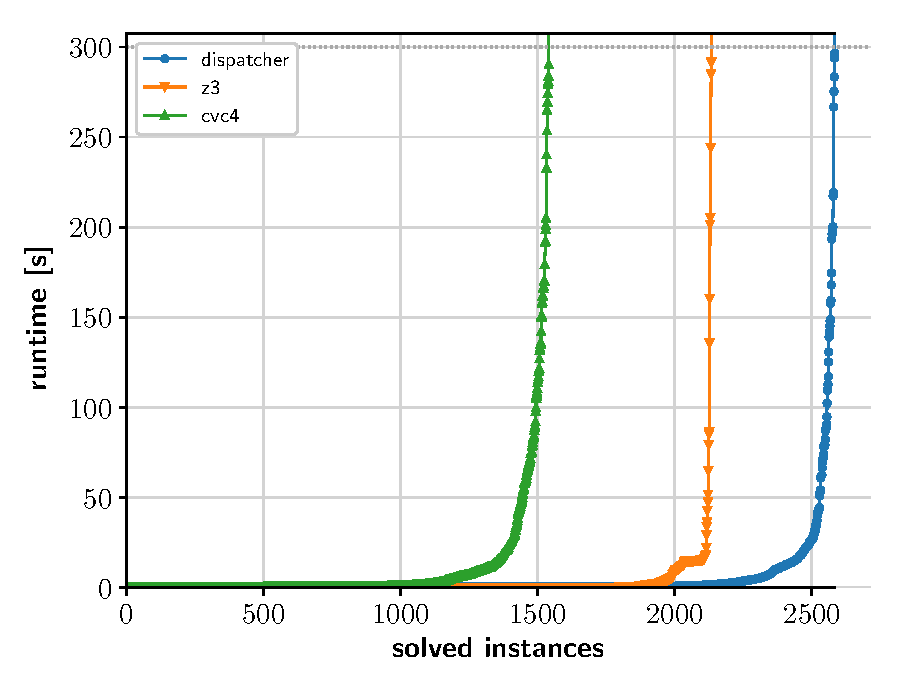
\includegraphics[width=.5\textwidth]{plot/cactus_qfnra_dispatcher_cvc4_z3}
&
\includegraphics[width=.5\textwidth]{plot/cactus_qfnia_dispatcher_cvc4_z3}  
\end{tabular}
\end{center}
\caption{\label{cactus}Cactus Plots comparing the dispatcher, Z3 and CVC4 on benchmarks from QF\_NRA and QF\_NIA.}
\end{figure}


\begin{figure}
\begin{center}
\begin{tabular}{cc}
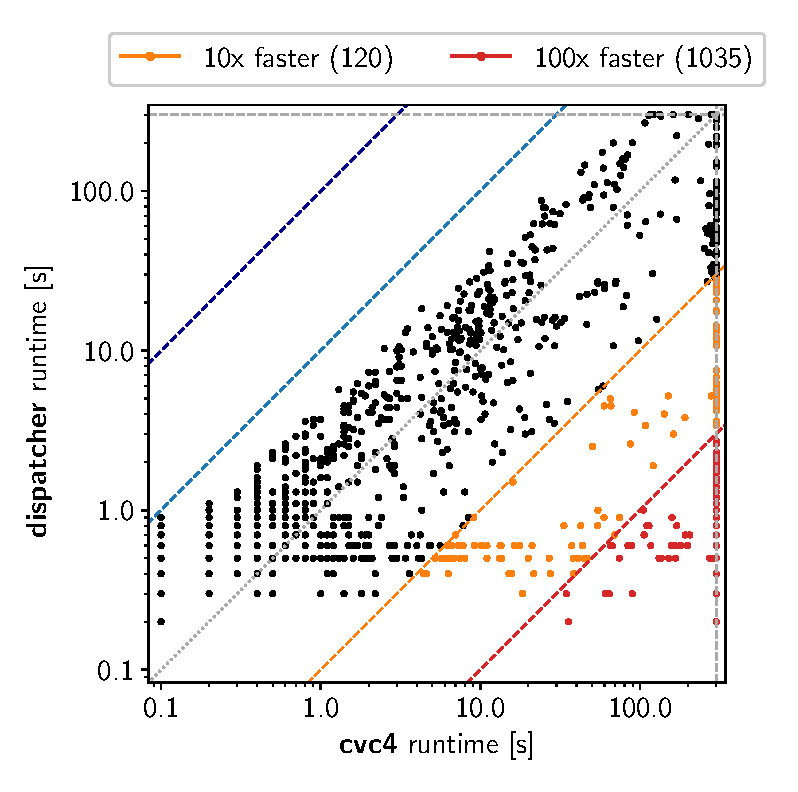
\includegraphics[width=.5\textwidth]{plot/scatter_qfnra_dispatcher_cvc4}
&
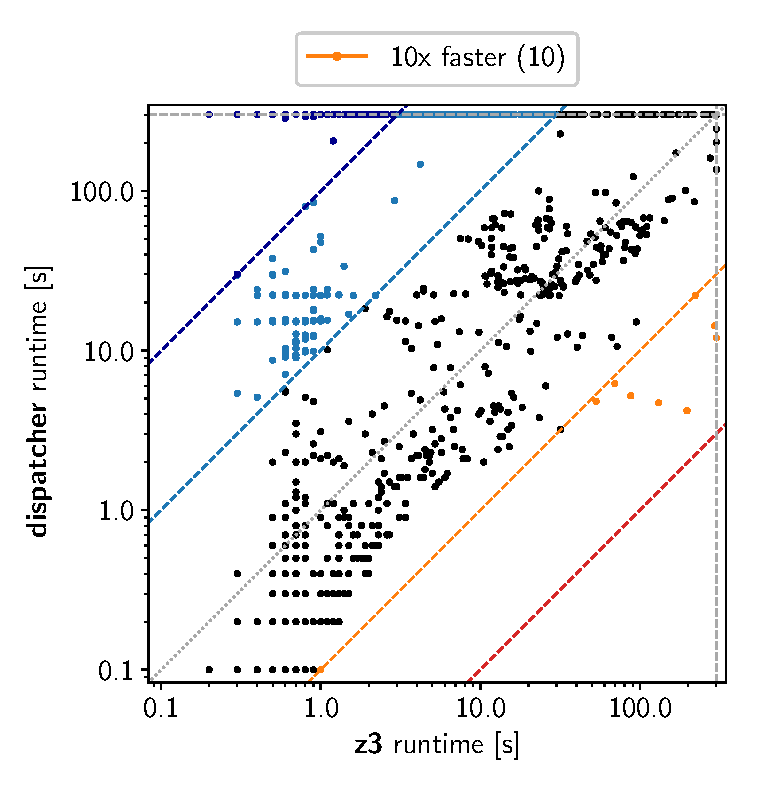
\includegraphics[width=.5\textwidth]{plot/scatter_qfnra_dispatcher_z3} 
\end{tabular}
\end{center}
\caption{\label{scatternra}Scatter plots comparing the dispatcher against Z3 and CVC4 on benchmarks from QF\_NRA.}
\end{figure}

\begin{figure}
\begin{center}
\begin{tabular}{cc}
\includegraphics[width=.5\textwidth]{plot/scatter_qfnia_dispatcher_cvc4}
&
\includegraphics[width=.5\textwidth]{plot/scatter_qfnia_dispatcher_z3}  
\end{tabular}
\end{center}
\caption{\label{scatternia}Scatter plots comparing the dispatcher against Z3 and CVC4 on benchmarks from QF\_NIA.}
\end{figure}

\bibliography{mybib}{}
\bibliographystyle{plain}

\end{document}
